\section{mSTS assembly and its services}
 The \gls{mSTS} comprises 11 modules (22 \glspl{FEB}) and 2 pulser boards. Each module consists of a silicon sensor, shielded microcables, and 2 \gls{FEB}s. Two different silicon sensor sizes were used to assemble \gls{mSTS} modules - 62 by 62 mm and 62 by 122 mm. Each side of the sensor has 1024 strips which are connected via microcables to the readout electronics - 8 STS-XYTERs on the \gls{FEB}. The microcables transport analog signals, but they can be influenced by any electromagnetic interference. The analog signal received by the chips is then amplified and converted into the digital domain. Subsequently, the digital signal is transported via the \gls{ROB}s (in total 5 readout boards - one in the \gls{mSTS} - one for each unit) to the \gls{CRI} and then processed and analyzed. In total \gls{mSTS} has 22 528 readout channels which constitute only 1.25 \% of the final detector. In order to avoid overheating and reduce noise, the \gls{FEE} needs to be properly cooled and powered which is discussed in section~\ref{msts_powering} and~\ref{msts_cooling}. 
\subsection{Powering}
\label{msts_powering}
The powering of the \gls{mSTS} is organized in a similar fashion as it will be implemented for the final \gls{STS} (see section~\ref{powering} and figure~\ref{fig_msts_scheme})~\cite{Koczon:2020Jc}. Each power board (in total 5 \glspl{POB} - one for each unit/C-frame) is populated with DC/DC converters (2.5 V and 3 V~\cite{DC_DC_converter}) is connected to the low voltage modules several meters away from the experiment site. The double-sided silicon sensors are symmetrically reverse-biased (\SI{75}{V} and \SI{-75}{V}) and operated in a constant voltage mode, each side of the sensor is connected to a high voltage module located in the same crate as the low voltage ones. The details of the powering scheme and the modules mounted on the carbon ladders can be seen in the figure~\ref{fig_msts_scheme}.

\begin{figure}[!h]
\centering
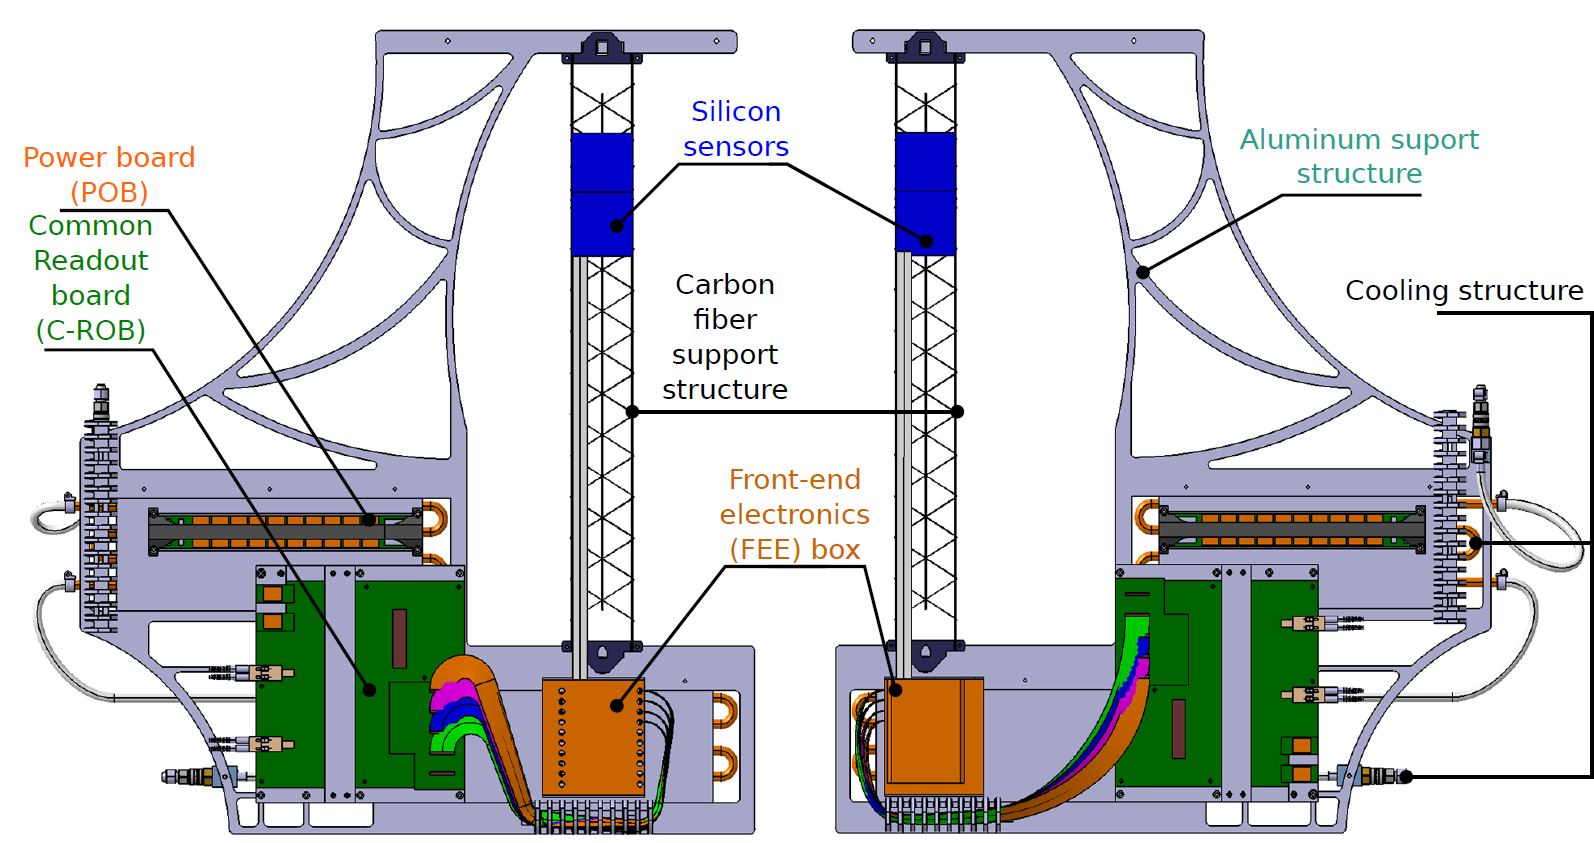
\includegraphics[width=0.8\columnwidth]{Chapter6/DCS/images/unit0.png}
\caption{Schematic view of the \gls{mSTS}'s first station}
\label{fig_msts_scheme}
\end{figure}
\newpage
\subsubsection{Noise considerations}
\footnote{Noise}{unwanted high-frequency disturbance or interference with the electrical signal} problems are the most common and critical issues while building a high-energy physics particle detector. The total noise contribution can be divided into four components~\cite{noise_twepp2008}:
\begin{itemize}
    \item thermal noise $n_{TH}(t)$ - contributions caused by the current passing through a resistor,
    \item \gls{EMI} in Detector-FEE connection, $n_{D-E}(t)$,
    \item \gls{EMI} in \gls{FEE}-external connections, $n_{E-F}(t)$,
    \item additional sources, related to the intrinsic noise of the FEE elements, $n_{add}(t)$.
\end{itemize}
From the practical point of view, designing and implementing a proper powering and grounding scheme play a critical role in the data quality from the detector~\cite{Bobillier:1159563}. The silicon sensors are characterized by very low signal levels and a significant number of channels, what makes them particularly sensitive to noise pickup. In the case of the \gls{mSTS}, the \gls{FEE} is located quite far away from the silicon sensor. The microcables connecting the two mentioned elements (sensor and \gls{FEB}) are shielded but the \gls{EMI} of the analog signal could be clearly observed when the cables are not completely flat (due to e.g. external stresses). The other contribution which is related to the noise picked up between the \gls{FEE} and external connections are addressed by for example adding an additional filter box (first order RC-filter) for the silicon sensor biasing lines. The total noise in the system serves as a reference for the minimum signal level that could be processed. More detailed considerations about the noise influence on the system are described in the section~\ref{module}. During the laboratory tests, satisfactory performance of the detector modules was achieved (\gls{ENC} of 1000~$e^{-}$). Nevertheless, the performance in the experiment area can differ greatly, due to devices belonging to other subsystems or the accelerator services. The problem with the noise performance of the modules was also identified in this case and substantial efforts were taken in order to find the noise sources and limit their influence (increasing the ADC threshold values of the STS-XYTERs). 

The \gls{mSTS}'s enclosure is decoupled from the experiment table (no direct connection of any conducting elements). The \gls{mSTS} enclosure is connected to a dedicated ground of the \gls{mCBM} experiment, preventing any \gls{EMI} on the lines that may affect the performance. In reality, there are no perfect grounds, even in the same line there might potential differences.  Figure~\ref{fig_msts_power} depicts the power distribution of the \gls{mSTS}. The floating ground scheme for the sensors biasing circuity and the front-end electronics come with important boundary conditions for the powering - each module side requires a separate powering line and the \gls{ROB} needs to be decoupled from the \gls{FEB} \cite{RodriguezRodriguez2020}. Moreover, to further reduce possible noise pickup a return path capacitor was implemented at the \gls{FEB} connectors and the \gls{HV} common return (depicted as C-RTN) was connected to the enclosure.
\begin{figure}[!h]
\centering
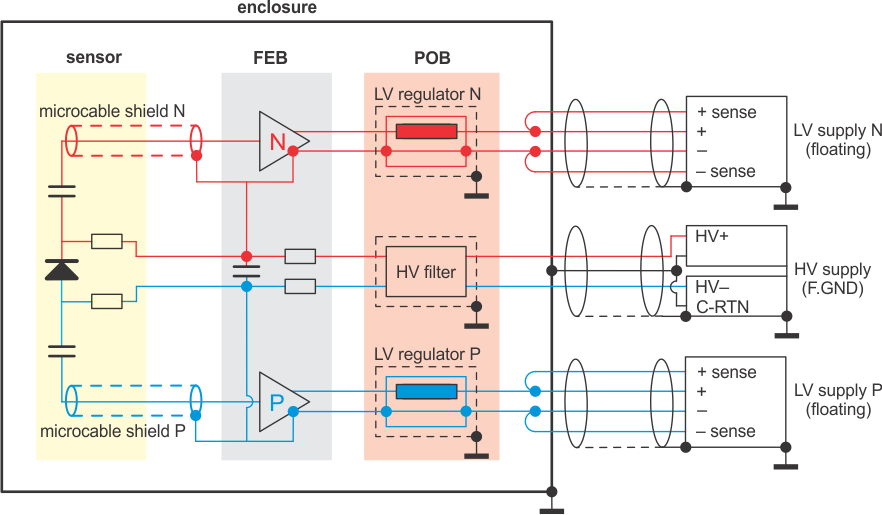
\includegraphics[width=0.75\columnwidth]{Chapter6/DCS/images/power_distribution.png}
\caption{Power distribution scheme of the \gls{mSTS} \cite{RodriguezRodriguez2020}}
\label{fig_msts_power}
\end{figure}
\newpage
\subsection{Cooling}
\label{msts_cooling}
In order to avoid overheating of the detector's \gls{FEE} and \glspl{POB}, the electronics need to be cooled. The cooling system for the \gls{mSTS} is a water-based cooling system, where the main heat exchange elements inside the detector are cooling plates.  Figure~\ref{fig_STS} shows the cooling plates which are thermally coupled to the fins with the \glspl{FEB}. Three Lauda chillers were used to pump chilled water through and efficiently evacuate excess heat. These chillers were also integrated into the control system via RS232-to-Ethernet converter. Figure~\ref{fig_cooling} depicts the bath temperature during the 430 days of operation. Initially, the \gls{mSTS} was cooled with two Lauda chillers. During the data taking in June 2022, one of the chillers failed due to radiation-induced damage. Since a similar chiller was unavailable, two other, less powerful units were employed. Therefore, values from the third cooling unit can be seen only during the last months of operation. The devices measure the temperature values, and the water that enters the detector is slightly higher (depending on the actual temperature in the experiment's location). Figure~\ref{fig_cooling} also shows the dew point inside the \gls{mSTS}, which should be always be below the water temperature, in order to avoid condensation on the \gls{FEE}.

\begin{figure}[!h]
\centering
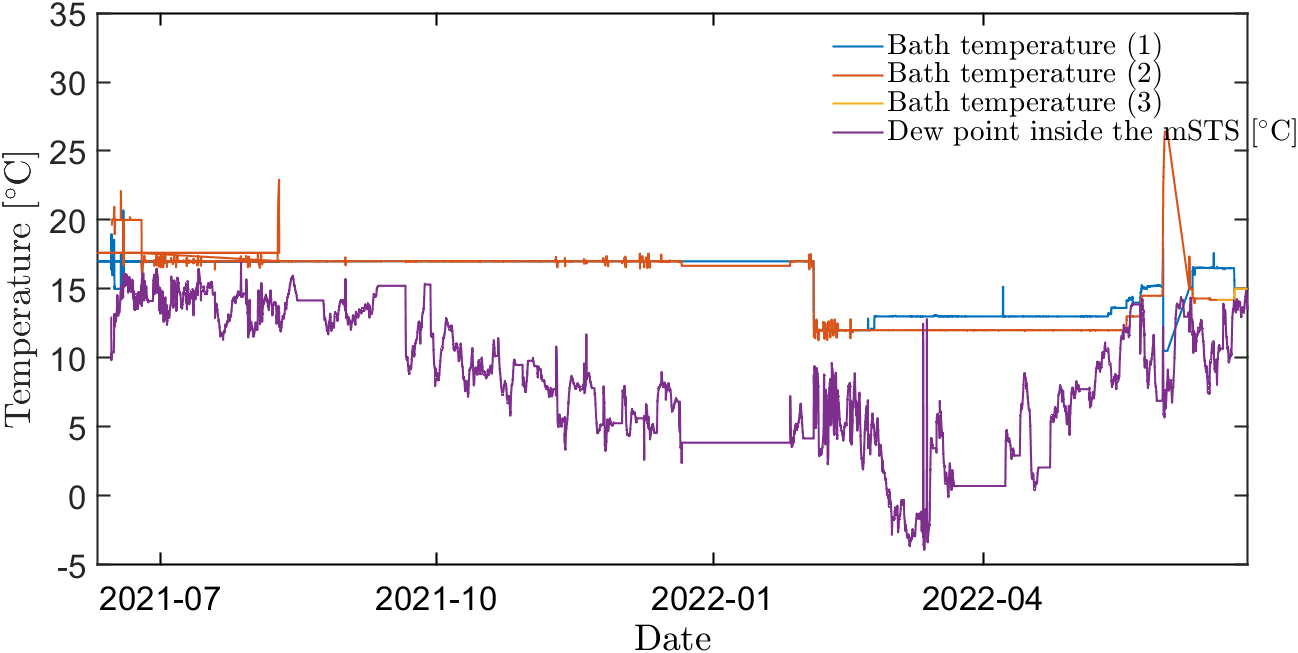
\includegraphics[width=0.6\columnwidth]{Chapter6/DCS/images/cooling.png}
\caption{Temperature readouts of the three Lauda chillers used for the \gls{mSTS} (denoted as 1, 2, 3) and the dew point inside the enclosure}
\label{fig_cooling}
\end{figure}
\newpage
\subsection{Detector modules}
 The modules differ in cable length, and sensor size, but also in components used to power them up, which may affect parameters like power dissipation or the general performance (different ENC levels).  The assembly of the detector is realized stepwise. The whole cumbersome procedure requires caution and precision. Therefore, a proper workflow was developed to address the complexity of the module assembly~\cite{carmen2}. This topic is more broadly discussed in the section \ref{module}. The respective components of each \gls{mSTS} unit can be found in the table~\ref{tab:msts_comp}. 

\begin{table}[!h]
\centering
\resizebox{\textwidth}{!}{%
\begin{tabular}{lllllll}
\hline
Unit & Ladder & Silicon sensors                                                                          & Microcables                                                      & \begin{tabular}[c]{@{}l@{}}DC/DC \\ converters\end{tabular} & \begin{tabular}[c]{@{}l@{}}STS-XYTER\\  version\end{tabular} & \gls{LDO} regulators             \\ \hline
0    & 0      & \begin{tabular}[c]{@{}l@{}}62x62 $mm^{2}$\\ 62x62 $mm^{2}$\end{tabular}                  & \begin{tabular}[c]{@{}l@{}}490 mm\\ 450 mm\end{tabular}          & 2.5 V, 3 V                                                  & 2.2                                                          & 1.8 V and 1.2 V            \\ \hline
$1^{*}$    & 0      & \begin{tabular}[c]{@{}l@{}}62x62 $mm^{2}$\\ 62x62 $mm^{2}$\end{tabular}                  & \begin{tabular}[c]{@{}l@{}}490 mm\\ 450 mm\end{tabular}          & 2.5 V, 3 V                                                  & 2.1                                                          & 1.8 V and 1.8 V with diode \\ \hline
2    & 0      & \begin{tabular}[c]{@{}l@{}}62x62 $mm^{2}$\\ 62x122 $mm^{2}$\end{tabular}                 & \begin{tabular}[c]{@{}l@{}}490 mm\\ 450 mm\end{tabular}          & 2.5 V, 3 V                                                  & 2.2                                                          & 1.8V and 1.2 V             \\ \hline
3    & 0      & \begin{tabular}[c]{@{}l@{}}62x62 $mm^{2}$\\ 62x62 $mm^{2}$\\ 62x62 $mm^{2}$\end{tabular} & \begin{tabular}[c]{@{}l@{}}490 mm\\ 450 mm\\ 420 mm\end{tabular} & 1.8 V, 2.4 V                                                & 2.1                                                          & 1.8 V and 1.8 V with diode \\ \hline
3    & 1      & \begin{tabular}[c]{@{}l@{}}62x122 $mm^{2}$\\ 62x122 $mm^{2}$\end{tabular}                & \begin{tabular}[c]{@{}l@{}}490 mm\\ 450 mm\end{tabular}          & 1.8 V, 2.4 V                                                & 2.1                                                          & 1.8 V and 1.8 V with diode \\ \hline
\end{tabular}%
}
\caption{mSTS units and differences between the components used for assembly (in order to achieve 1.2 V output, 1.8 V \gls{LDO} regulator was used with a diode)}
\label{tab:msts_comp}
\end{table}
\newpage
Before assembling the \gls{mSTS}, extensive measurements of all the building blocks were performed. Figure \ref{fig_msts_ENC1} and  \ref{fig_msts_ENC2} show measurements of two modules from different units. Unit 1 is the only unit used before for the previous \gls{mCBM} campaign~\cite{heuser1}. It is one of the oldest units and it's also slightly irradiated, therefore sensors' leakage current is elevated in comparison to the new modules. An example of modules testing can be seen in the figures \ref{fig_msts_ENC1} and \ref{fig_msts_ENC2}. The module of unit 1 (Figure \ref{fig_msts_ENC2}) has larger noise and odd-even effect than unit 0 module. Moreover, in both modules, the Z-strips (p-side channel numbers 0 to 128) are clearly recognizable. Figure \ref{fig_msts_ENC2} shows the theoretical ENC values for the building blocks of a module (sensor, microcables, and ASICs). The targeted \gls{ENC} value is 1000~$e^{-}$, nevertheless the measurement outcome depends also on the sensor size, microcables length and nuances of the assembly process. In case of \gls{mSTS} modules the targeted \gls{ENC} value was achieved during the laboratory testing, but from the obtained data and the ADC thresholds used during the data-taking campaign we can conclude that the \gls{ENC} levels were higher than 1000~$e^{-}$.%\newpage
\begin{figure}[h!]
\centering
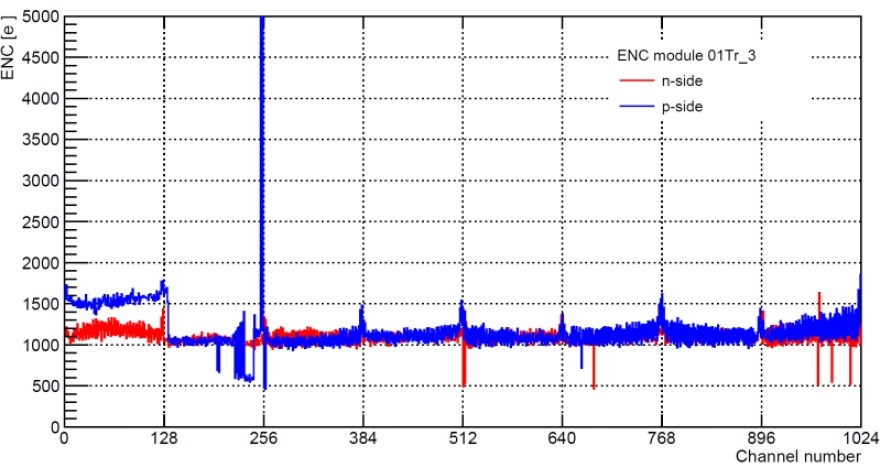
\includegraphics[width=0.6\columnwidth]{Chapter6/DCS/images/U0M1_ENC.jpg}
\caption{Equivalent Noise Charge for module 0 of unit 1~\cite{RodriguezRodriguez2020}}
\label{fig_msts_ENC1}
\end{figure}

\begin{figure}[h!]
\centering
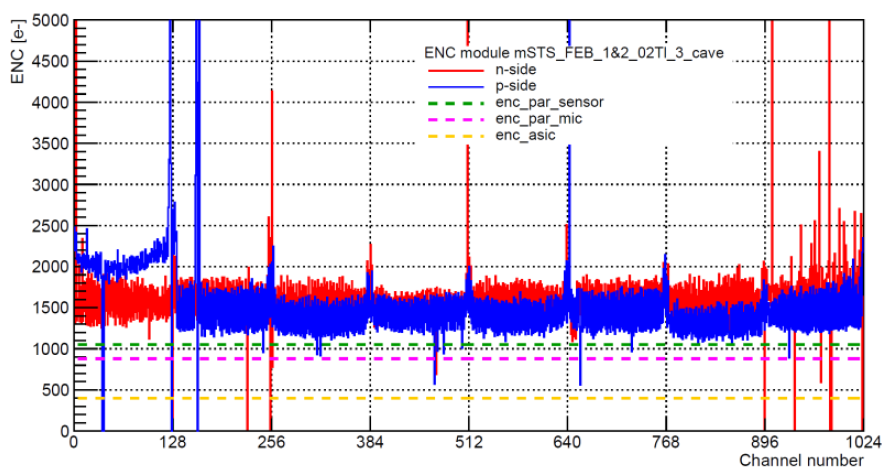
\includegraphics[width=0.6\columnwidth]{Chapter6/DCS/images/U1M1_ENC.png}
\caption{Equivalent Noise Charge plots for module 0 of unit 0~\cite{RodriguezRodriguez2020}}
\label{fig_msts_ENC2}
\end{figure}
\newpage
\subsection{Installation of the mSTS}
Figure \ref{fig_msts_state} depicts the assembly process of the \gls{mSTS}. Before transferring the detector to the \gls{mCBM} experiment modules of every unit were thoroughly tested:
\begin{itemize}
    \item before ladder assembly,
    \item after installation on the unit,
    \item after assembling the c-frame in the mSTS enclosure.
\end{itemize}
The detector services (\gls{LV}, \gls{HV}, cooling) patch panel was installed on the front wall of the \gls{mSTS} enclosure~\cite{tekli1}. At that point the detector was ready to be transferred to the experiment area and the commissioning began.

\begin{figure}[h!]
\centering
\includegraphics[width=0.99\columnwidth]{Chapter6/DCS/images/msts_all.png}
\caption{Assembly process of the \gls{mSTS} (from left to right)}
\label{fig_msts_state}
\end{figure}
%\newpage
 The first photo on the left side depicts the first c-frame after installing it inside the detector's enclosure. The second photo shows one of the last stages of the detector assembly, all detector modules are mounted. The last photo shows the detector after its transfer to the experiment cave and the last checks related to detector services. %\newpage

\section{Operation of the mSTS}

The \gls{mSTS}'s \gls{DCS} is a fairly automatized system in which monitoring and control are taken care of by the Finite State Machine. An operator, that is most likely the person tackling the data acquisition system, should monitor leakage current, temperatures, dew point, availability of the nodes as well as the overall system state (based on the \gls{FSM}). All the logs are available either in Phoebus or Kibana. Moreover, the alarm server together with Phoebus takes care of notifying the operator about alarms (exceeding limits, communication errors, etc.). This section contains the summary of the most important findings which were obtained through the \gls{DCS}. 
\subsection{Power dissipation of the mSTS}
 Power consumption of the 11 modules (22 \glspl{FEB}) of the \gls{mSTS} was studied in detail to better understand the differences between the modules and estimate how predictions meet the experimental results. The values obtained through the \gls{mSTS} were compared with the measurements of two frond-end boards and average values from modules calibration. In order to compare the results, the \gls{CSA} (front and back register) of all STS-XYTERs were changed to values from 7 to 42 with a step of 5.
 
 Figure \ref{fig_power_scheme} depicts the power dissipation of different components based on the \gls{CSA} value for measurements conducted with a separate pair of \gls{FEB}s. These two \glspl{FEB} were powered directly using a \gls{LV} power supply (R\&S~HMP4040). The power dissipation estimations for the distribution lines and the DC/DC converters were performed based on the assumed efficiency of 80 \%, which might be lower for $I > 2$~A dropping down to 65~\% at \SI{10}{\celsius} with currents approaching the device output limit (3~A). In this case, due to the settings of the \glspl{ASIC} the currents for the digital line were slightly higher than expected for the operation - around 2.3~A instead of 1.9~A. The analog line currents are defined by the \gls{CSA} register values and in this case varied from 1.4~A to 4.1~A.  Due to the experimental nature of the \gls{mSTS} and its powering scheme, the voltage drop of every element in the distribution lines can't be determined accurately. Therefore, the calculations made for the distribution lines based on the currents measured for the \glspl{FEB} and modules can't be considered as a reference. A detailed description of the powering scheme can be found in section~\ref{module}.  For this estimation, a constant value of voltage drop in the \gls{LDO} regulators of 0.6~V was assumed. 

 
\begin{figure}[h!]
\centering
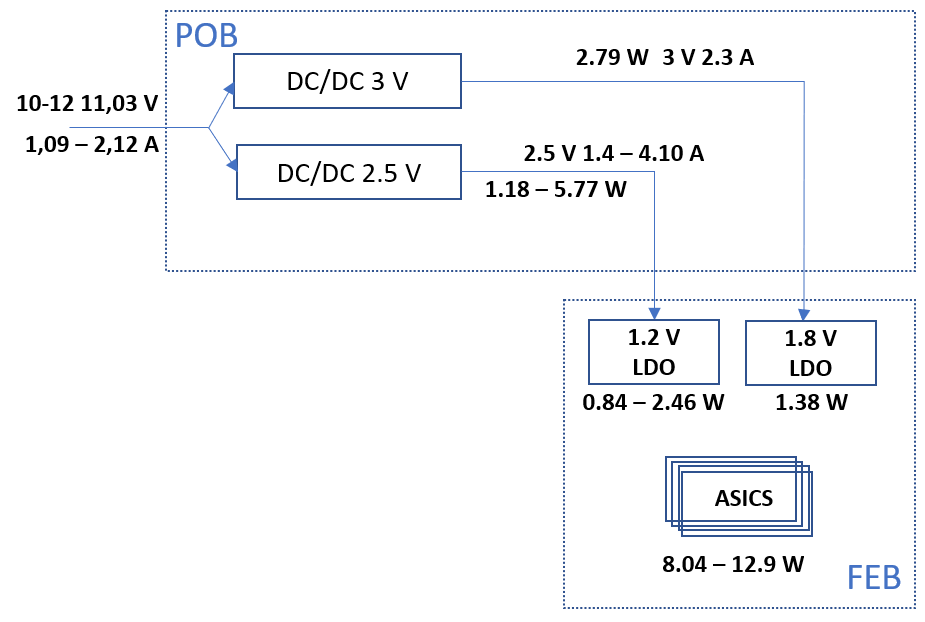
\includegraphics[width=0.65\columnwidth]{Chapter6/DCS/images/POB.png}
\caption{mSTS's powering scheme with power dissipation estimations for different components depending of the \gls{CSA} value set}
\label{fig_power_scheme}
\end{figure}


The pie charts in the figure \ref{fig_power_CSA} show that while increasing the power consumption of the \gls{ASIC}s we also significantly increase the share of the power dissipated by the DC/DC converters and distribution lines. %\newpage
\newpage
\begin{figure}[h!]
\centering
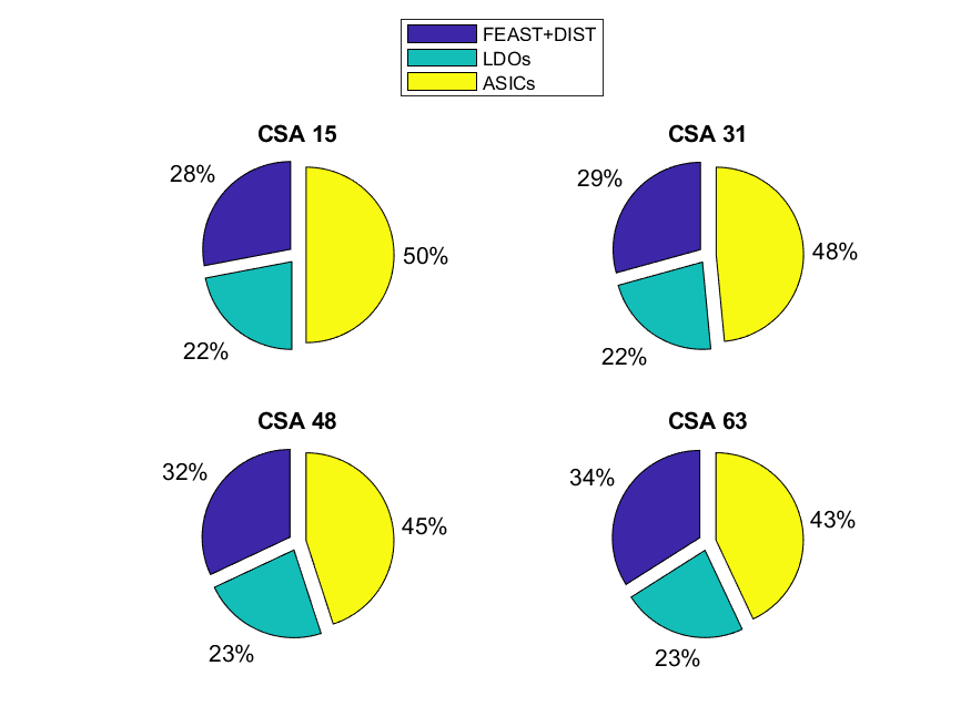
\includegraphics[width=0.65\columnwidth]{Chapter6/DCS/images/POBpie.png}
\caption{Power dissipation share of different components of the powering scheme depending on the \gls{CSA} value}
\label{fig_power_CSA}
\end{figure}
Figure \ref{fig_power2} shows the current drawn by 4 \glspl{FEB} of unit 1 depending on the \gls{CSA} value. It was determined that the \gls{CSA} value of 31 should be the nominal value for the \gls{STS} modules, as it is a default value for the STS-XYTERv2.2 and this value also ensures that the signal amplification is correct (\gls{CSA} value of 31 corresponds to 2~mA per analog channel). Nevertheless, the \gls{CSA} value may vary to address the different needs of modules (depending for example on their noise levels).  Moreover, the DC/DC converter responsible for powering the analog front end (\gls{AFE}) is limited to the 3~A, therefore also the higher values of \gls{CSA} won't lead to higher current in the circuit.
%\begin{figure}[h!]
%\centering
%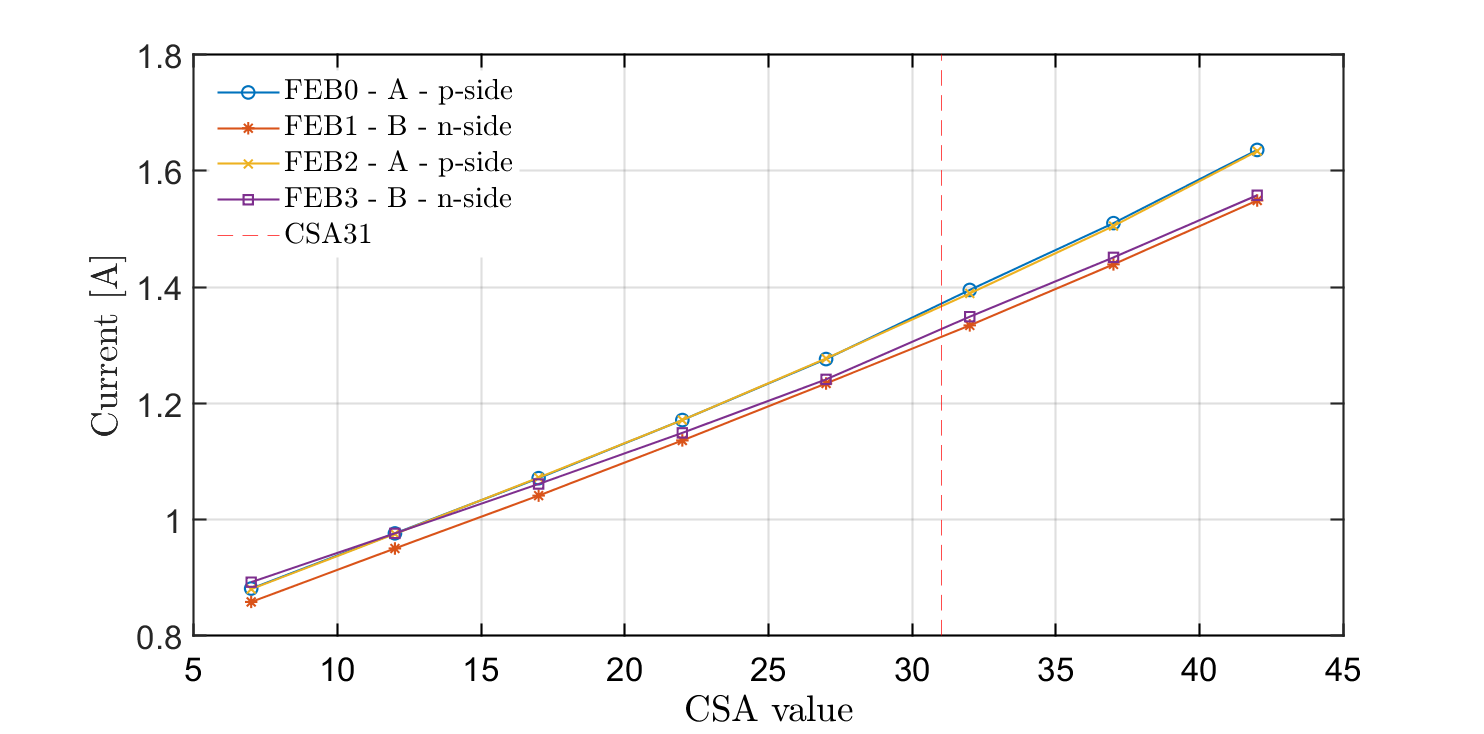
\includegraphics[width=0.45\columnwidth]{Chapter6/DCS/images/U0CSABIAS.png}
%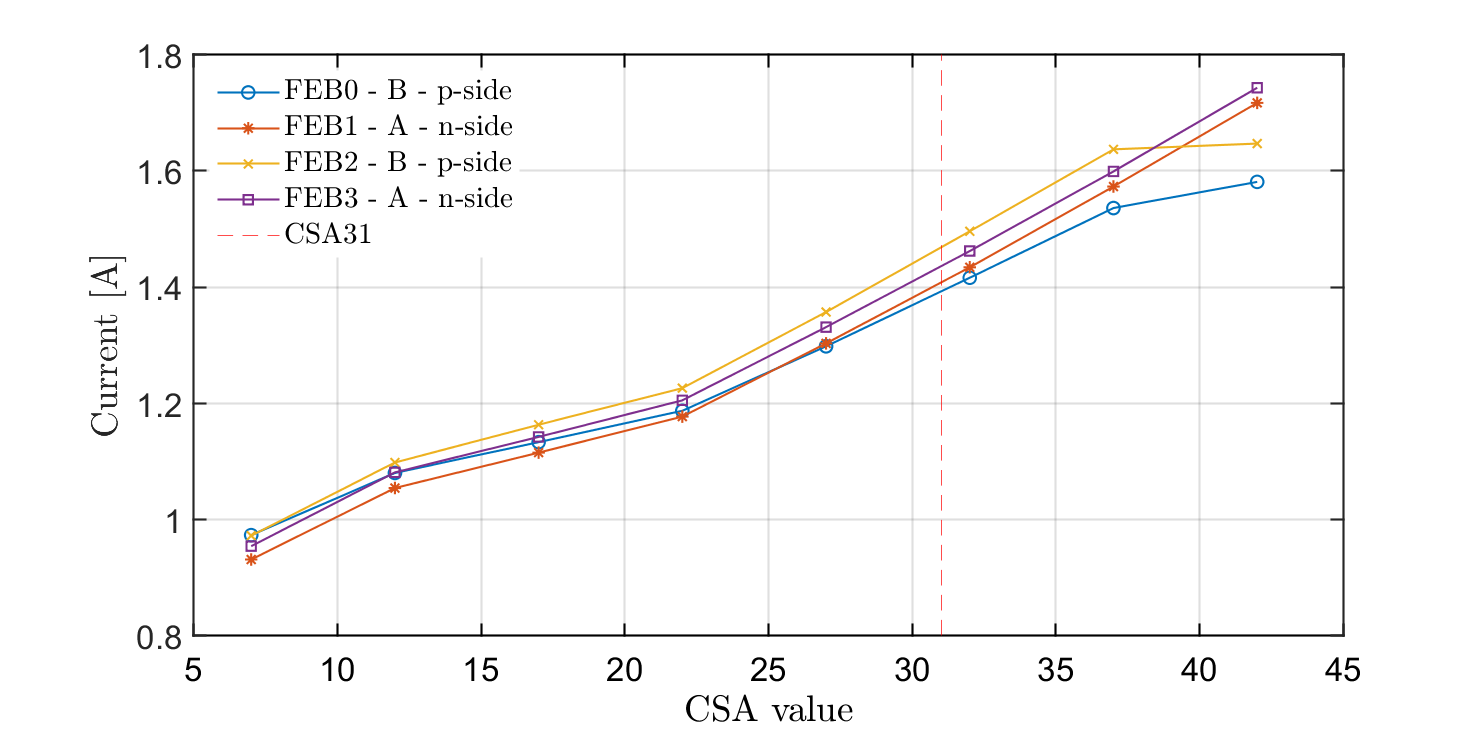
\includegraphics[width=0.45\columnwidth]{Chapter6/DCS/images/U1CSABIAS.png}
%\caption{CSA scan of the unit 0 (left) and 1 (right)}
%\label{fig_power1}
%\end{figure}

\begin{figure}[h!]
\centering
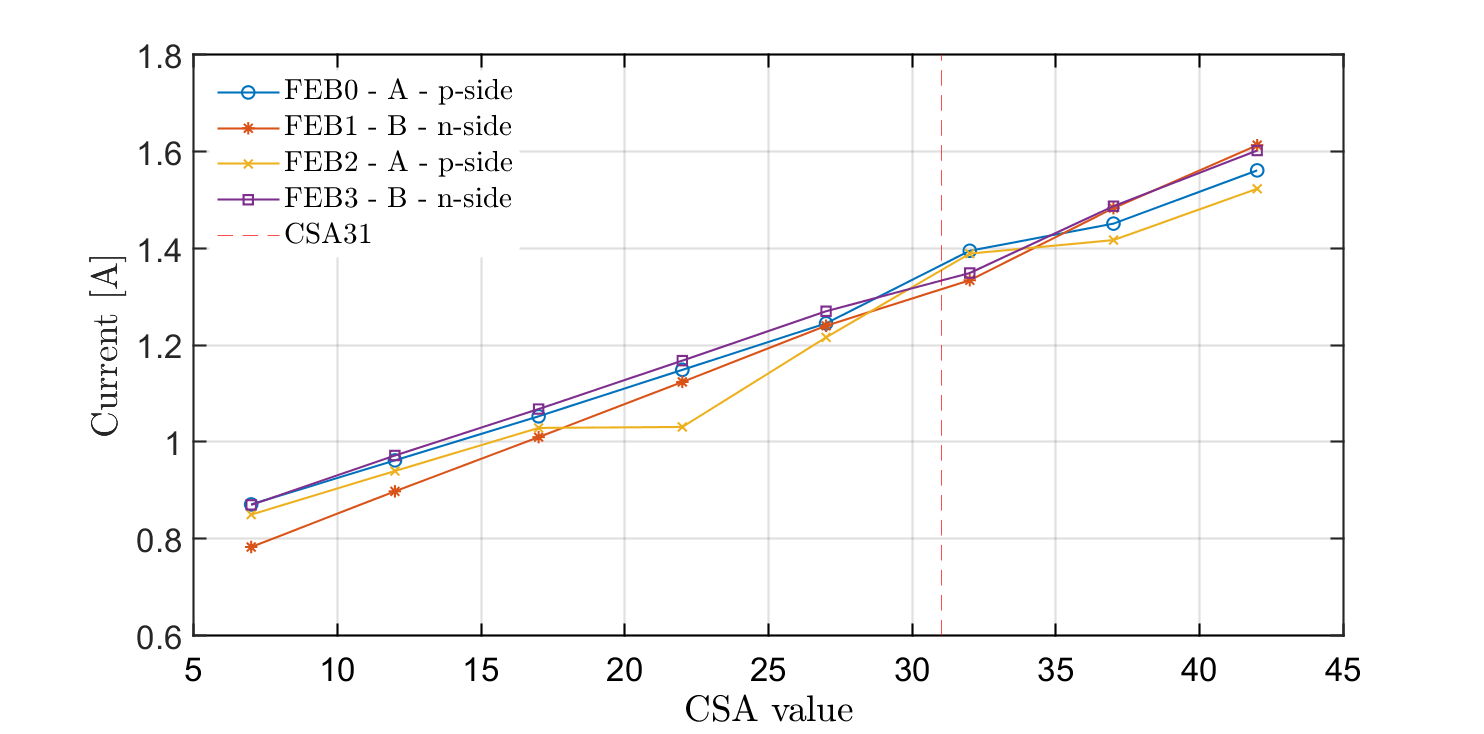
\includegraphics[width=0.45\columnwidth]{Chapter6/DCS/images/U2CSABIAS.png}
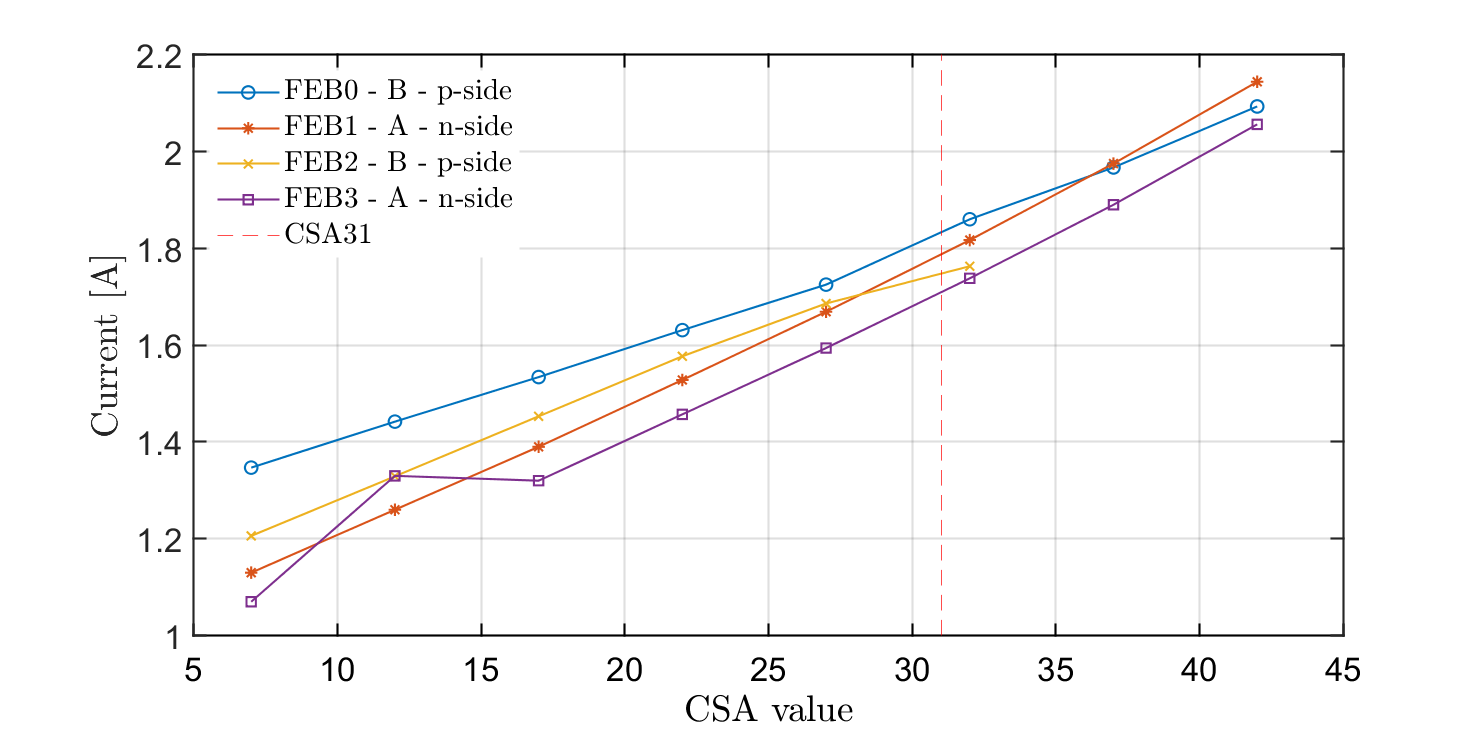
\includegraphics[width=0.45\columnwidth]{Chapter6/DCS/images/U3L1CSABIAS.png}
\caption{CSA scan of the unit 2 (left) and unit 3 ladder 0 (right)}
\label{fig_power2}
\end{figure}
\newpage
Similar measurements were also conducted for all the other \gls{mSTS} modules (see Appendix~\ref{CSA}). The average values of the current (a module is powered by two low voltage channels) for every unit are depicted in the figure \ref{fig_avg}. For the older modules, especially those powered by 1.8 V and 2.4~V DC/DC converters (Unit 3), the currents are significantly higher, reaching 1.6 - 1.8~A for the \gls{CSA} 31. The \gls{AFE} of the unit 1 modules are powered by the 1.8~V \gls{LDO} regulators with a diode, which causes a voltage drop of approximately 0.6~V. Nevertheless, this sub-optimal solution can be also seen via increased current and power dissipation of the unit 1 modules. The current of modules of units 0 and 2 are similar, as they use the same components, which are also considered the final parts for the \gls{STS}.

%\newpage
\begin{figure}[h!]
\centering
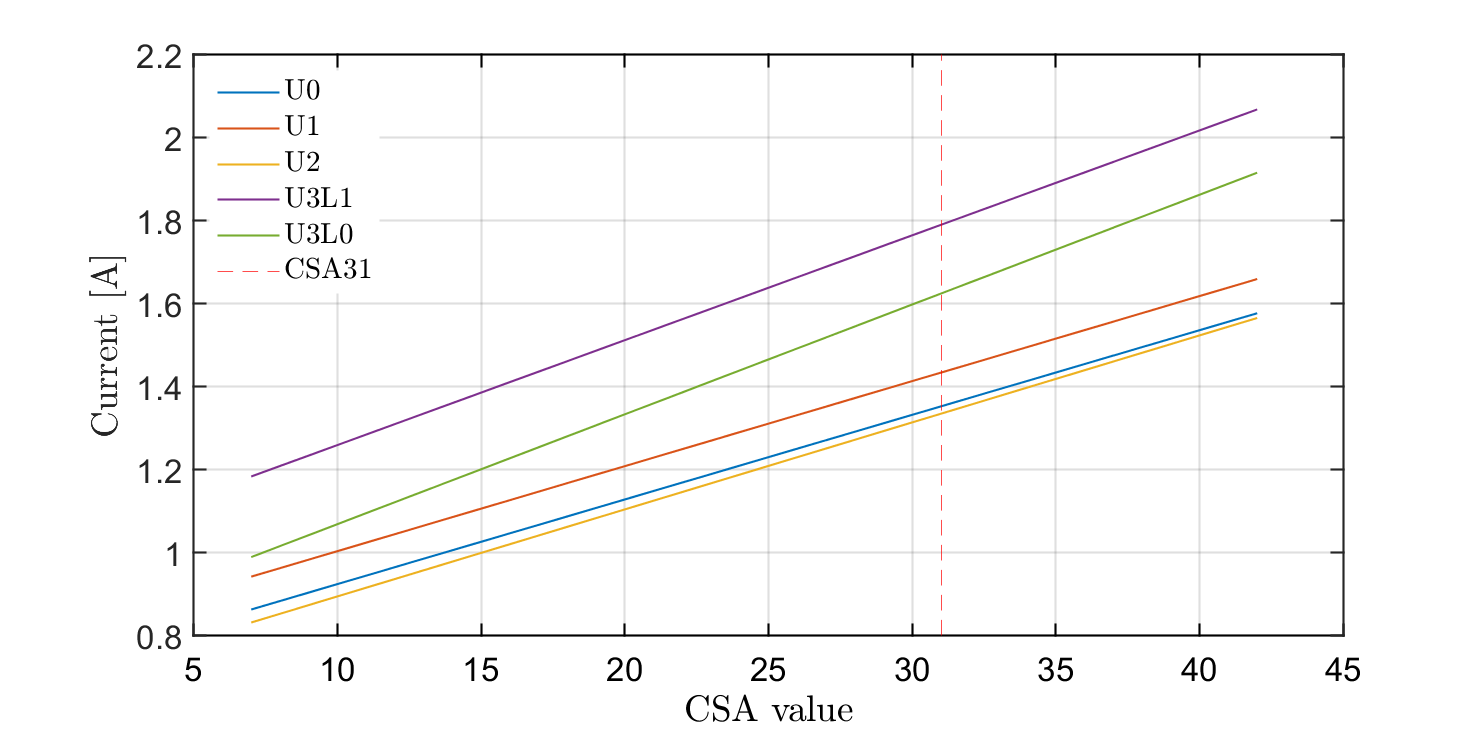
\includegraphics[width=0.6\columnwidth]{Chapter6/DCS/images/units.png}
\caption{Average current of each \gls{mSTS} unit}
\label{fig_avg}
\end{figure}

The modules are powered in the constant voltage mode, which means that the output voltage is always 10.5~V. Knowing the currents at the power supply level, cable lengths, and voltage drops on subsequent components, the power estimation can be made based on the equation:
\begin{equation}
    P = VI
\end{equation}
Moreover, we can also try to estimate the power consumption based on the values from the module testing prior to the detector assembly. Average values of the currents are presented in the \ref{tab:typical_cons}. By adding estimates related to the distribution lines and DC/DC converters from figure~\ref{fig_power_scheme} we can compare the results with the \gls{mSTS} results. 
\begin{table}[!h]
\centering
\begin{tabular}{lll}
\hline
CSA & Current digital {[}A{]} & Current \gls{AFE} {[}A{]} \\ \hline
15  & 1.9                 & 1.02                    \\
31  & 1.9                 & 2.05                    \\
48  & 1.9                 & 3.07                    \\
63  & 1.9                 & 4.10                    \\ \hline
\end{tabular}
\caption{Currents supplied to the analog front end and to the digital part depending on the set \gls{CSA} value}
\label{tab:typical_cons}
\end{table}
\newpage
Figure \ref{fig_theor} shows the comparison of the power consumption of \gls{mSTS} units with the calculations based on the average current from the modules testing (depicted as FLA v2) and FEB currents (denoted as FLA). The values obtained from the calculation follow unit 1 power consumption. 

\begin{figure}[h!]
\centering
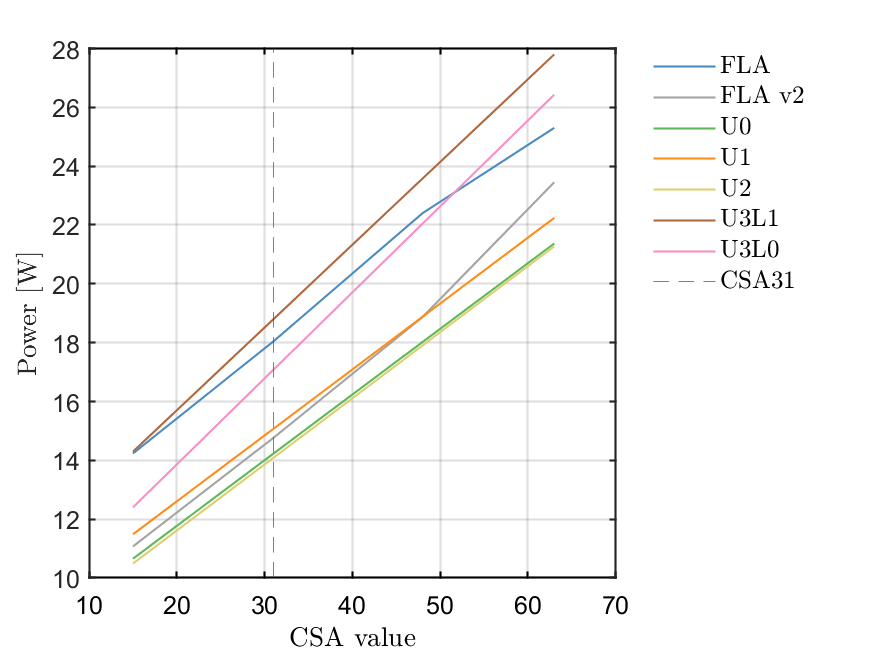
\includegraphics[width=0.65\columnwidth]{Chapter6/DCS/images/theor.png}
\caption{Average power dissipation of the units compared with predictions based on theoretical power dissipation in the components (depicted as FLA)} 
\label{fig_theor}
\end{figure}
The components used for units 0 and 2 are considered to be almost the final ones, therefore the power consumption of these modules should serve as a reference for further calculations. Some parameters related to the voltage drop may change, mostly due to different powering lines' lengths and diameters, as well as different connectors. 
\begin{table}[h!]
\centering
\begin{tabular}{lll}
\hline
               & \gls{CSA} 31  & \gls{CSA} 48  \\ \hline
FLA estimation & 31.5 kW & 38.8 kW \\
Unit 3         & 32.9 kW & 41.3 kW \\
Unit 2         & 24.7 kW & 29.9 kW \\ \hline
\end{tabular}
\caption{Total power consumption of the 876 modules of the \gls{STS} based on the calculations from the figure~\ref{fig_theor}}
\label{tab:power_cons}
\end{table}
Therefore, the values stated in the table~\ref{tab:power_cons} can't be considered as a reference. Nevertheless, they give a good estimation of the power consumption and also show how the module assembly evolved. 
%\newpage
\subsection{Parameters monitoring and obtained data}
All the software and hardware components mentioned in the previous sections deliver essential information about the detector's safety and health. Thanks to the ongoing ambient monitoring many features of the subsystem were discovered and addressed, e.g. not sufficient cooling. Figure \ref{fig_temp} shows the temperature trends during the 450 days of operation. The first sensor (depicted in blue) was placed at the top of the \gls{mSTS}'s enclosure, and the second one (depicted in orange) is located on the upper part of unit 2. Temperatures registered in the \gls{mSTS} vary not only depending on the \gls{FEE} powering (peaks observed throughout the period) but also on the temperature in the cave. Moreover, the broader peak at the end of the depicted period is associated with the cooling unit's failure.  There are also a few periods, with the longest in December and January, when the detector was not operated. 

\begin{figure}[!h]
\centering
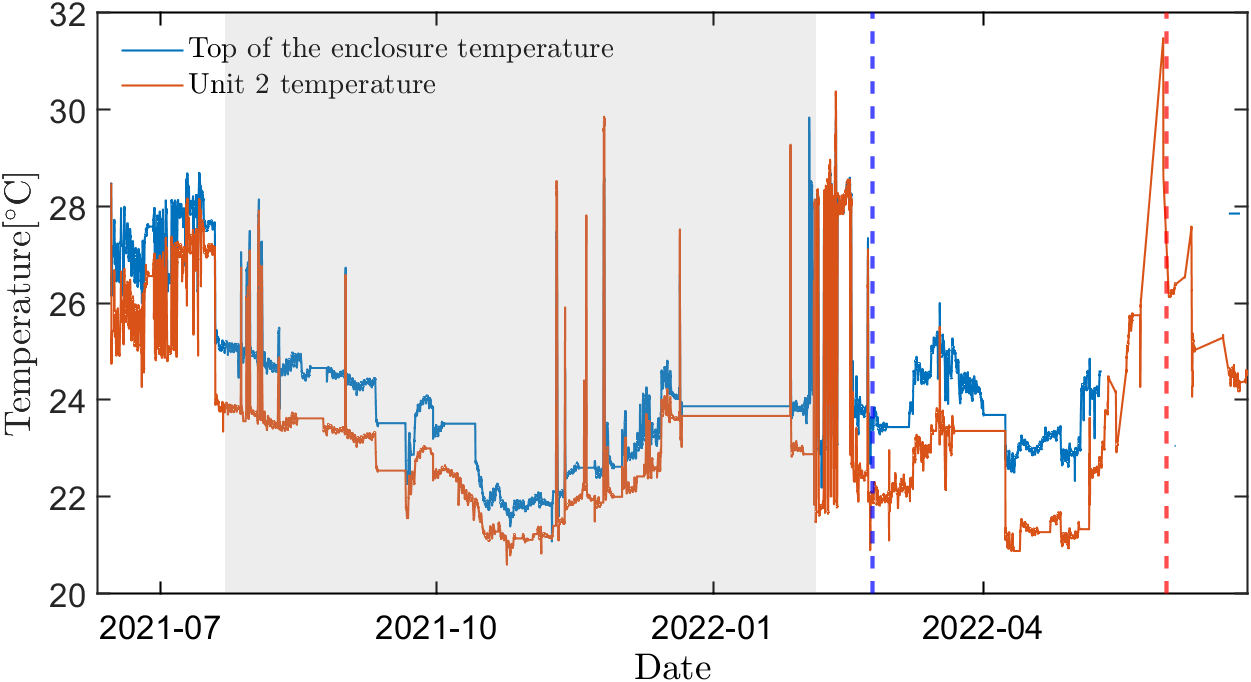
\includegraphics[width=0.55\columnwidth]{Chapter6/DCS/images/temp2.png}
\caption{Temperature monitoring}
\label{fig_temp}
\end{figure}

To ensure the safe operation of the system, it's also necessary to have information about the dew point. Water condensation on the parts of the \gls{FEE} could cause a whole ladder to fail. Figure \ref{fig_dew} depicts the differences in the dew point and temperature over the mentioned period. The coolant setpoint was always carefully adjusted depending on the situation in the experiment cave. 
\newpage
\begin{figure}[!h]
\centering
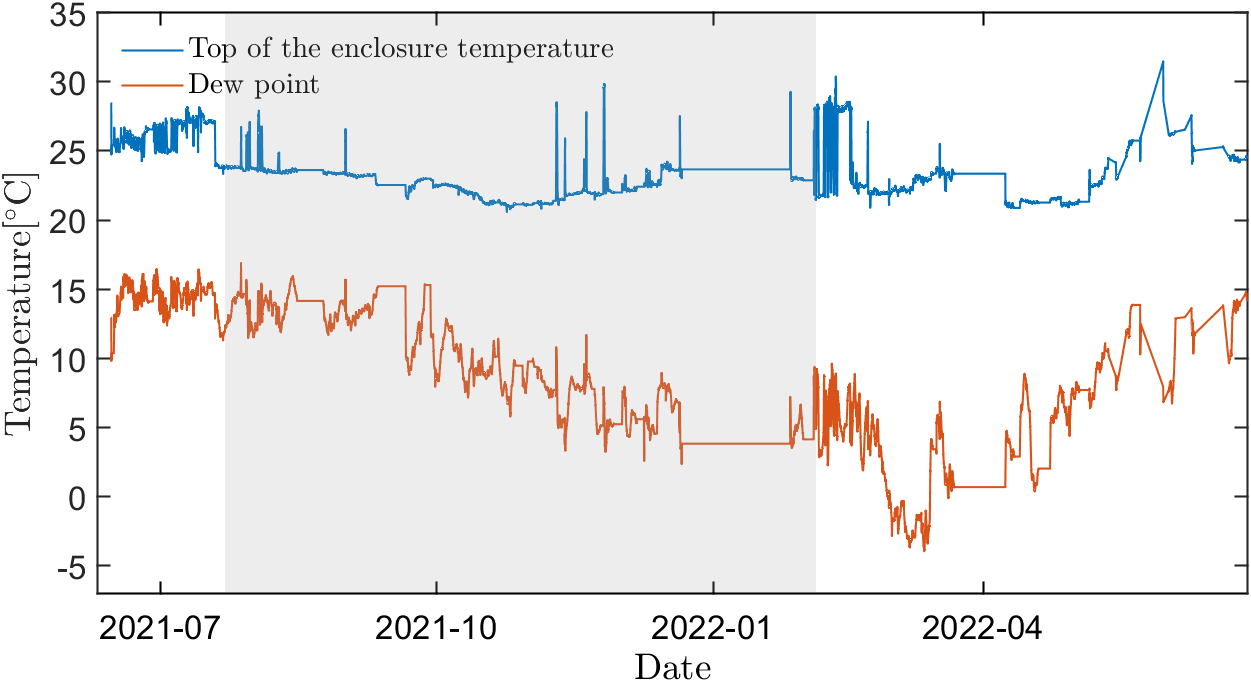
\includegraphics[width=0.55\columnwidth]{Chapter6/DCS/images/dew.png}
\caption{Temperature and dew point monitoring}
\label{fig_dew}
\end{figure}


Apart from ambient temperature and humidity monitoring, temperature sensors are also used to monitor the temperature on the powering boards. A comparison of the temperature on the \gls{POB} of unit 1, 2 and between two POBs of unit 3 are presented in the figure~\ref{fig_POB1}. Temperature measured in the unit 3, especially at the beginning of the operation, were much higher than those measured in unit 0 and 1. This effect is associated with a cooling issue which was resolved at the beginning of 2022. At the right end of the plot, we can see again the cooling unit failure. 
\begin{figure}[!h]
\centering
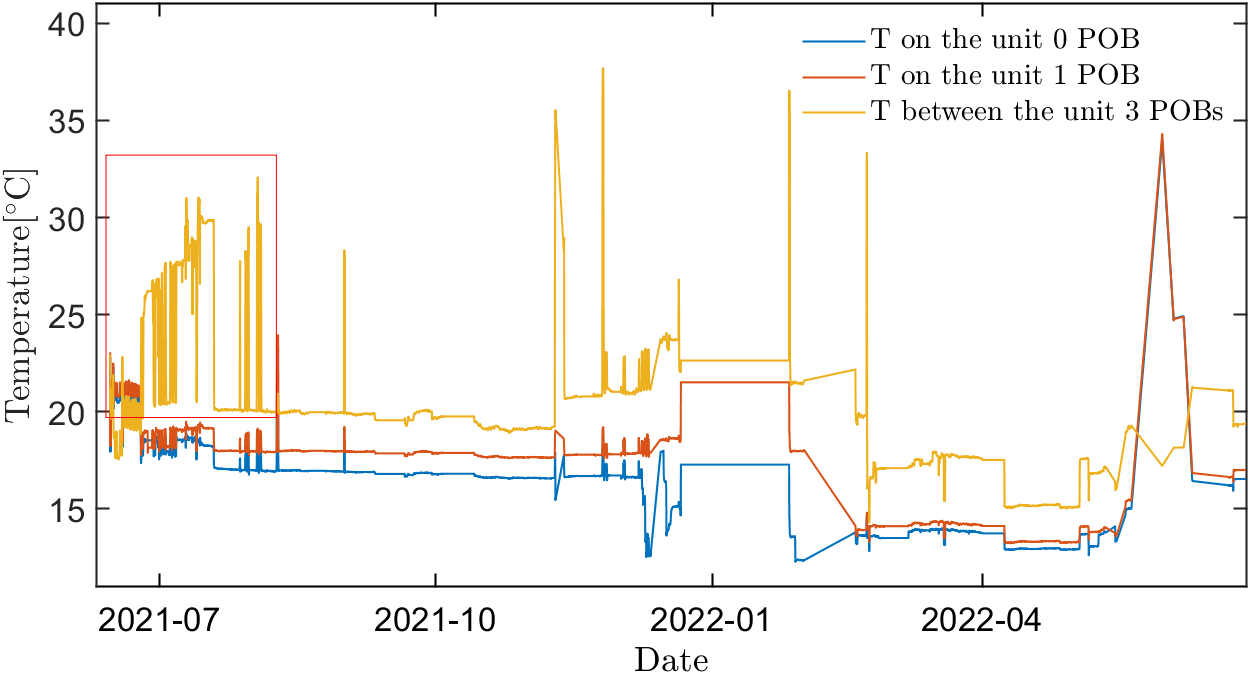
\includegraphics[width=0.55\columnwidth]{Chapter6/DCS/images/POB1.png}
\caption{Temperature on the POBs enclosure}
\label{fig_POB1}
\end{figure}
\newpage
Moreover, the temperature on the \gls{ROB} and \gls{FEB} was monitored, as depicted in the figure~\ref{fig_robvsfeb}. Interestingly, the temperature on the \gls{ROB} is higher than the temperature on the \gls{FEB} box on the unit 2. Unit 2 features 2 modules, 4 \gls{FEB}s (+ pulser board) in the \gls{FEB} box (each drawing about 1.6 A at constant 10.5 V), in comparison to the \gls{ROB} which is powered with 7 V and consumes about 0.8 A. This is, most likely, related to the position of better contact of the \gls{FEB} box to the cooling plate.

\begin{figure}[!h]
\centering
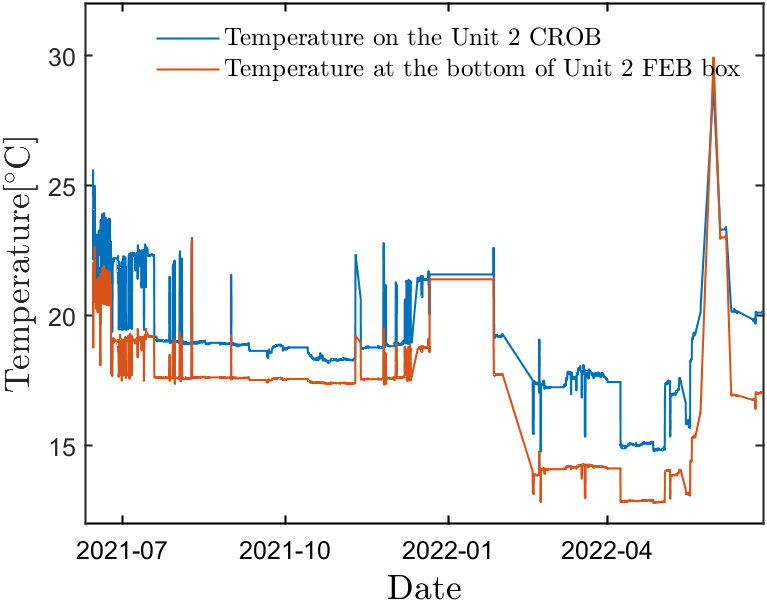
\includegraphics[width=0.55\columnwidth]{Chapter6/DCS/images/ROBvsFEB.png}
\caption{Temperature on the \gls{ROB}, \gls{FEB} box}
\label{fig_robvsfeb}
\end{figure}

\subsection{Monitoring of the leakage current}

Information about the temperatures serves not only to ensure detector safety but also to understand the behavior of the silicon sensors properly. Especially when analyzing and comparing the leakage current of the sensors, the temperature is of high importance as it allows the normalizing of the current to the same value. Firstly, if the exact temperature characteristic of the sensors is now known, it's necessary to rely on a temperature sensor placed close to the semiconductor. In the \gls{mSTS} several sensors are measuring ambient conditions, an overview can be seen in figure \ref{fig_temperatures}. The temperature inside the detector is significantly lower, which indicates that the cooling is working. Higher temperatures are also seen on the top of the detector. 

\newpage
\begin{figure}[!h]
\centering
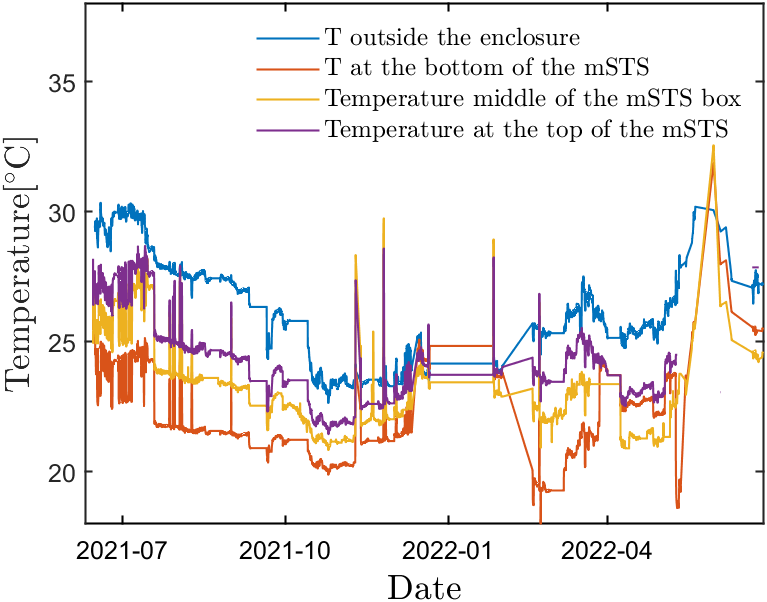
\includegraphics[width=0.55\columnwidth]{Chapter6/DCS/images/rates/tempmSTS.png}
\caption{Distributions of the temperatures inside the \gls{mSTS}}
\label{fig_temperatures}
\end{figure}

As the silicon sensors are reverse-biased, the nominal operating voltage was chosen to be $\pm75$ (as the full depletion of the non-irradiated silicon sensors is assured). The reverse polarity implies also negative current values. Nevertheless, only one side or channel will be discussed. The other side of the sensor is characterized by the same trends, but opposite sign.

%\newpage
\begin{figure}[!h]
\centering
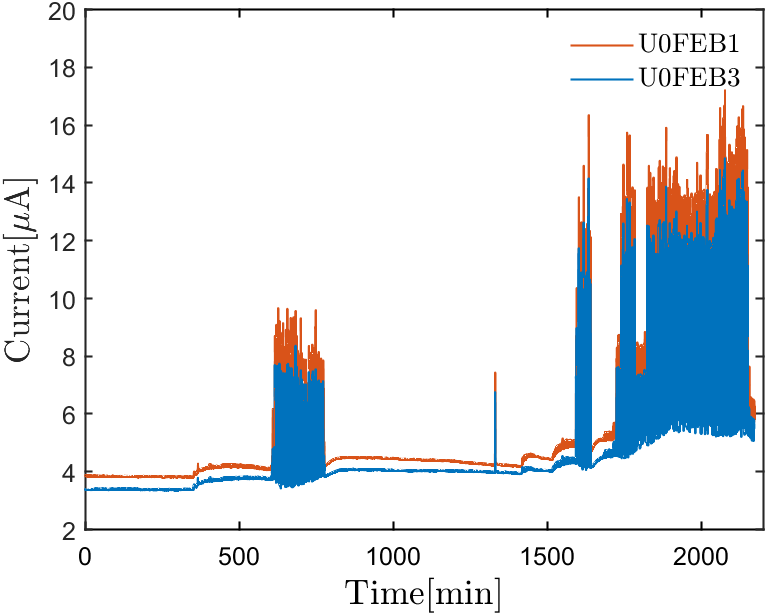
\includegraphics[width=0.45\columnwidth]{Chapter6/DCS/images/uranium/U0.png}
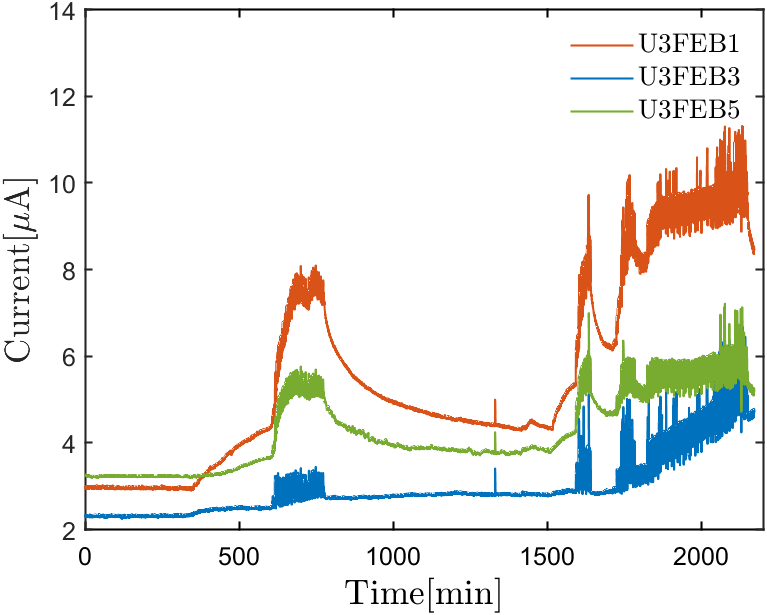
\includegraphics[width=0.45\columnwidth]{Chapter6/DCS/images/uranium/U3.png}
\caption{Leakage current of the silicon sensors in modules of units 0 and 3 during collisions of uranium with the gold target of different thicknesses.}
\label{fig_msts_LC}
\end{figure}

Typical behavior of the \gls{STS} silicon sensors during data-taking can be seen in figure~\ref{fig_msts_LC}. Due to radiation-induced surface and bulk damage, the leakage current will increase with the increasing total fluence that the sensors were exposed to. In order to properly compare the leakage current before and after the irradiation it's necessary to have the same ambient conditions or to measure the temperature and then normalize the current to \SI{20}{\celsius}. Apart from the constant leakage current rise during the data-taking, two particular parts of the plot can be distinguished. The first one just after 500 minutes when increased beam intensity leads to disclosing the spill structure. A similar trend can also be observed from around 1500 min until the end. The sensors of different units behave differently, depending on their position relative to the beam or sensor size, electrical short circuits.


\begin{figure}[!h]
\centering
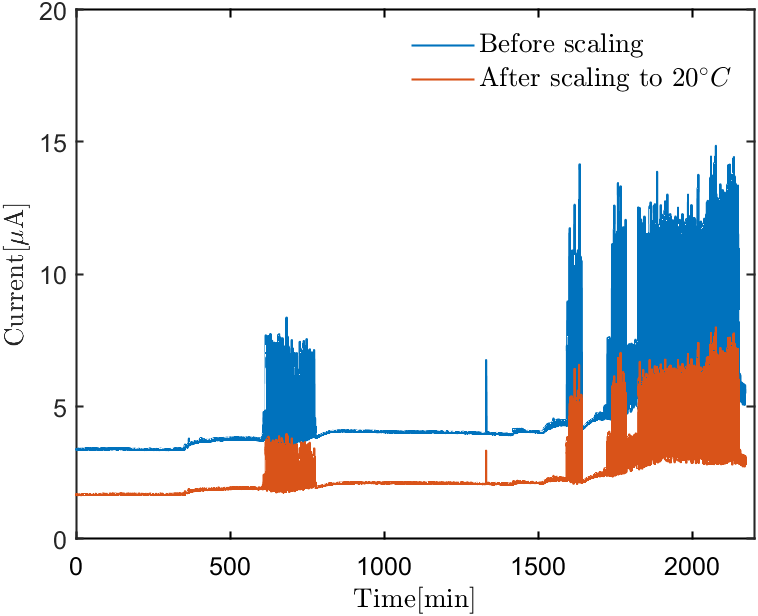
\includegraphics[width=0.45\columnwidth]{Chapter6/DCS/images/uranium/current_U_highintensity.png}
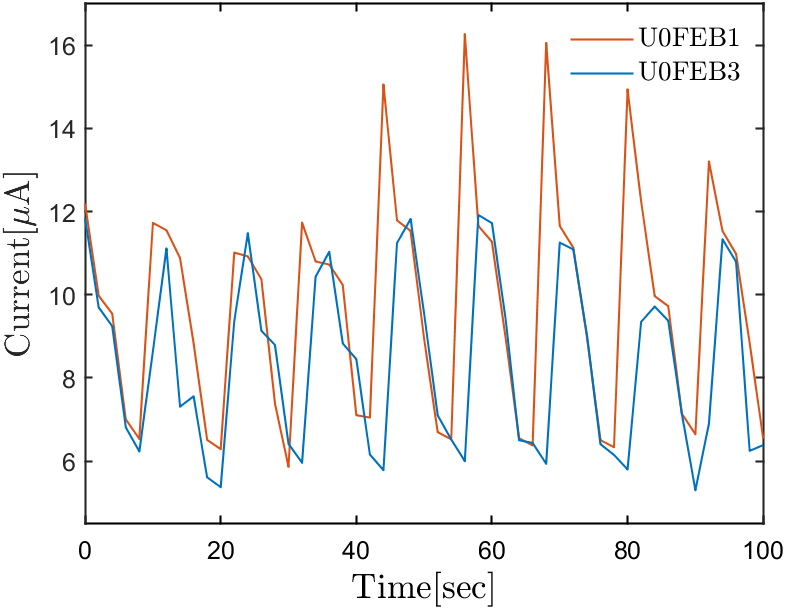
\includegraphics[width=0.47\columnwidth]{Chapter6/DCS/images/uranium/U3L1_spill.png}
\caption{Unit 0 \gls{FEB} 3 - normalization of the current (left) and zoomed-in view of the spill structure seen by the silicon sensors (10 s spill)}
\label{fig_sensors_spill}
\end{figure}

An example of the normalization of the unit 1 sensors is depicted in the figure~\ref{fig_sensors_spill}. A more detailed view of the spill structure is shown on the right plot. It can be clearly seen, that the reaction products traversing the silicons cause a significant leakage current increase of about \SI{10}{\micro A} (for the highest beam intensities - $10^{9}$ ions/s). Comparison of two units leakage current which was scaled to $20\,^{\circ}$C is shown in figure \ref{fig_leak}. Throughout the year 2021, only a few beam time campaigns took place, therefore leakage current increase due to radiation-induced damage is negligible. On the other hand, during the beam campaigns of 2022, the effect of radiation can be clearly seen.

\begin{figure}[!h]
\centering
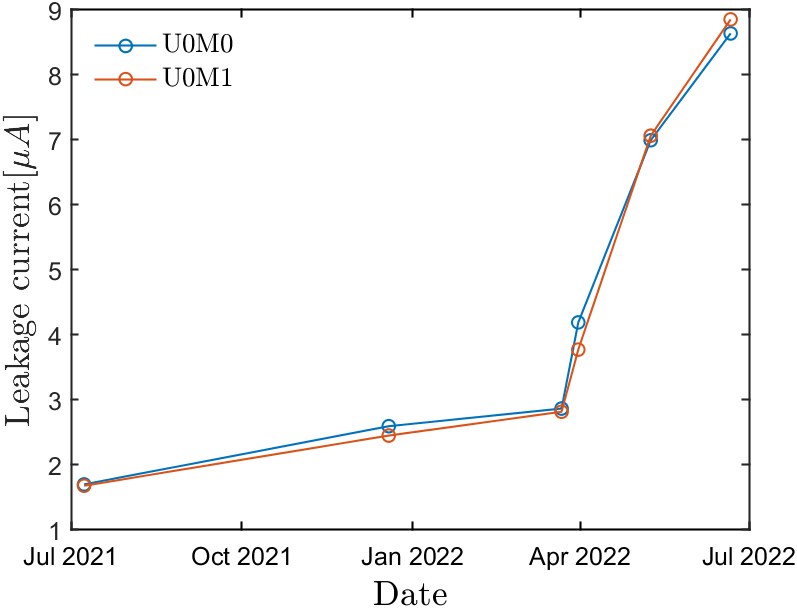
\includegraphics[width=0.45\columnwidth]{Chapter6/DCS/images/sensors/U0_leakage.png}
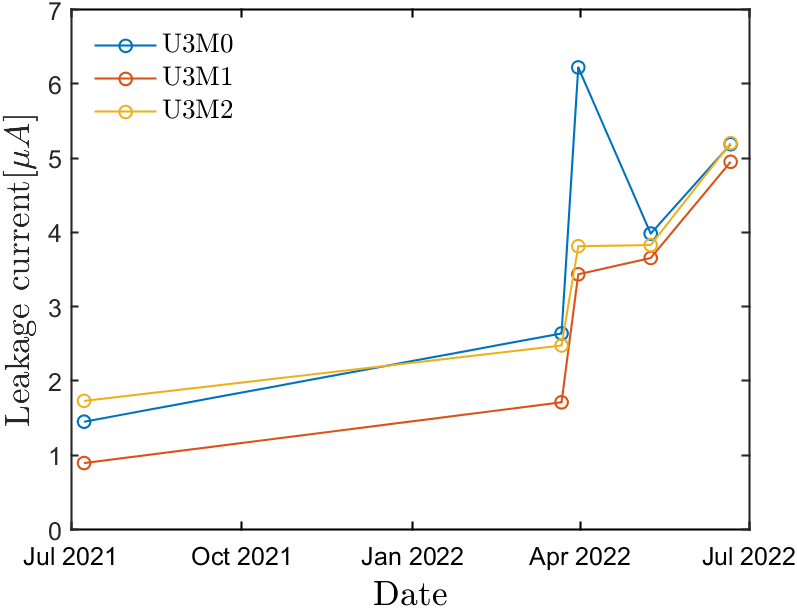
\includegraphics[width=0.45\columnwidth]{Chapter6/DCS/images/sensors/U3_leakage.png}
\caption{Leakage current evolution of the \gls{mSTS} sensors over the whole period of operation}
\label{fig_leak}
\end{figure}

\newpage
The quantitative current changes over the \gls{mCBM} campaign are shown in the table~\ref{tab:msts_final_fluence}. To better understand the overall results, it's important to take a look at the position of the silicon sensors with respect to the beam (see~figure~\ref{fig_sensors_scheme}). The sensors located closer to the collision point (from unit 0) are more irradiated than sensors from units 2 and 3. Furthermore, the results obtained from unit 3 are inconsistent throughout the experiment, which means that those modules are considered to have electrical issues (e.g. short circuits).


\begin{table}[!h]
\centering
\begin{tabular}{lcc}
\multicolumn{1}{c}{Module} & \begin{tabular}[c]{@{}c@{}}Current \\ difference {[}uA{]}\end{tabular} & Fluence {[}n/cm2{]} \\ \hline
U3L1M0                     & 16.23                                                                  & $2.5*10^{11}$          \\
U3L1M1                     & 7.6                                                                    & $5.8*10^{10}$          \\ \hline
U3L0M0                     & 3.7                                                                    & $5.7*10^{10}$          \\
U3L0M1                     & 4.1                                                                    & $6.2*10^{10}$          \\
U3L0M2                     & 3.5                                                                    & $5.3*10^{10}$          \\ \hline
U2M0                       & 3.6                                                                    & $5.5*10^{10}$          \\
U2M1                       & 6.3                                                                    & $4.8*10^{10}$          \\ \hline
U1M0                       & 6.4                                                                    & $9.8*10^{10}$          \\
U1M1                       & 6                                                                      & $9.1*10^{10}$          \\ \hline
U0M0                       & 6.9                                                                    & $1.1*10^{11}$          \\
U0M1                       & 7.2                                                                    & $1.1*10^{11}$         
\end{tabular}
\caption{Leakage current differences and corresponding fluence estimations for all the \gls{mSTS} modules.}
\label{tab:msts_final_fluence}
\end{table}

\begin{figure}[!h]
\centering
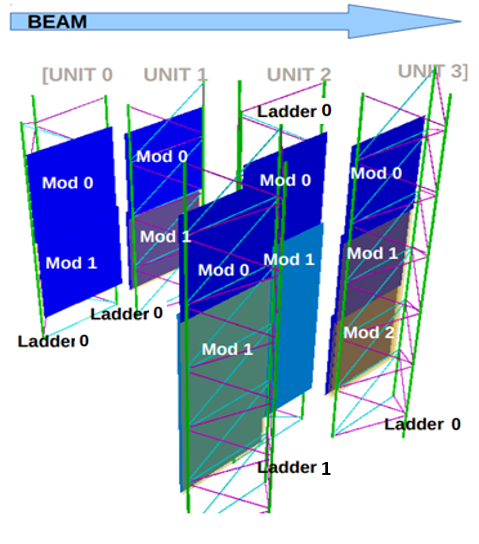
\includegraphics[width=0.4\columnwidth]{Chapter6/DCS/images/msts_sensors_scheme.png}
\caption{Schematic view of the \gls{mSTS} sensors position with respect to the beam}
\label{fig_sensors_scheme}
\end{figure}
\newpage
\subsection{IV characteristic of chosen modules}
The IV curves provide crucial information about the detector performance (see section \ref{sensors}):
\begin{itemize}
    \item shot noise, closely related to the leakage current which increases with the fluence,
    \item type inversion,
    \item annealing and reverse annealing,
\end{itemize}
Figure \ref{fig_IV} shows IV curves of two modules from two different units (1 and 3). 
\begin{figure}[!h]
\centering
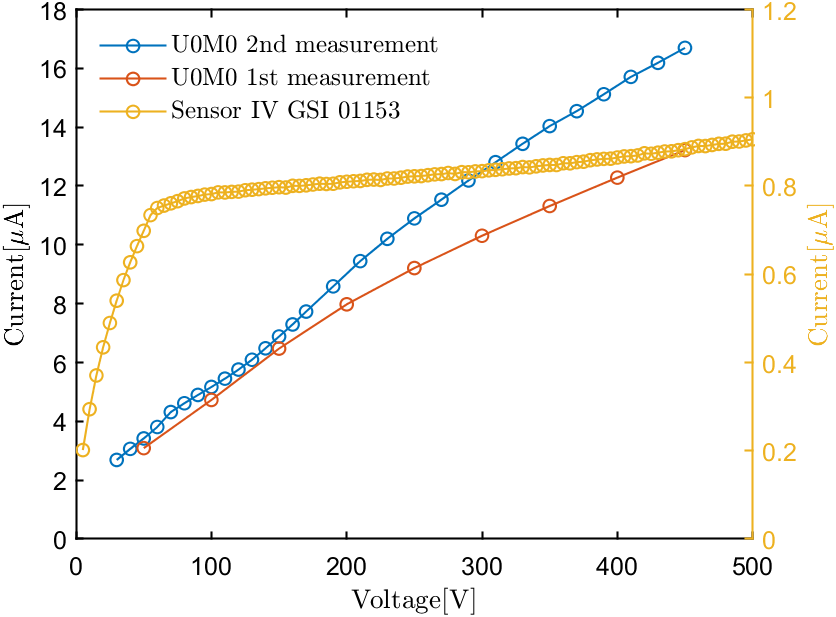
\includegraphics[width=0.45\columnwidth]{Chapter6/DCS/images/IV/U0FEB1.png}
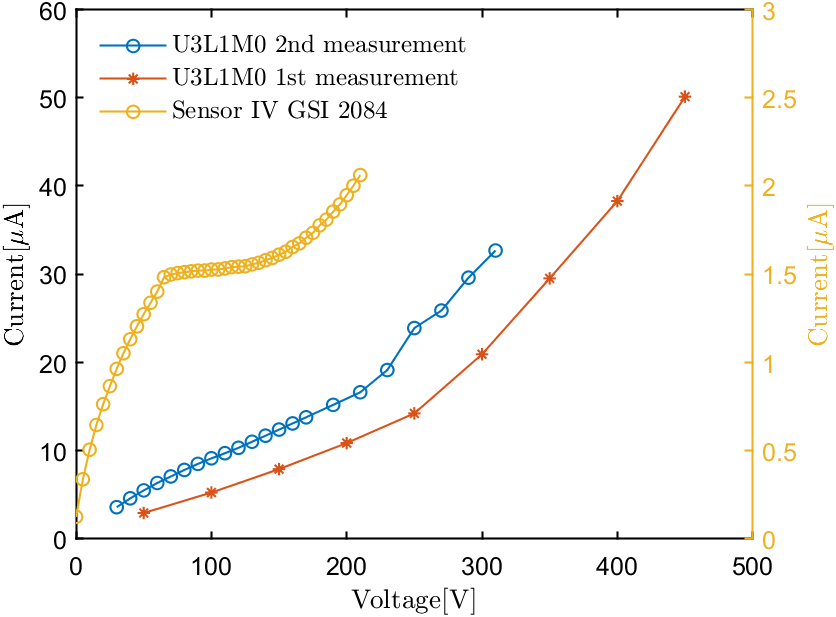
\includegraphics[width=0.45\columnwidth]{Chapter6/DCS/images/IV/U3L1FEB1.png}
\caption{IV curves for two modules from different units}
\label{fig_IV}
\end{figure}

The leakage current is scaled down to $\SI{20}{\celsius}$ but the relative humidity was different for each measurement. The IV measured during the QA procedure before the assembly of the module is depicted in yellow and shows a typical behavior of a revers-biased silicon diode with a full depletion reached around 60-70~V. The two other IV measurements for each module took place after assembly in the \gls{mSTS}, the beam campaign with the uranium beam, and the end of data-taking for 2022. The linear behavior of the sensors can be seen after the module assembly, measuring with an external high-voltage filter in a floating scheme. Nevertheless, the unit 3 sensor shows breakdown at similar biasing voltage for all three measurements. Figure~\ref{fig_IV_good} shows the IV measurement of a module without additional \gls{HV} filter and a Keithley power supply instead of Wiener \gls{LV} module. The \gls{HV} filter was integrated in the new version of the \gls{FEB} (FEB8-3), therefore new measurements will take place to establish the behavior of the module with the new PCB.

\begin{figure}[!h]
\centering
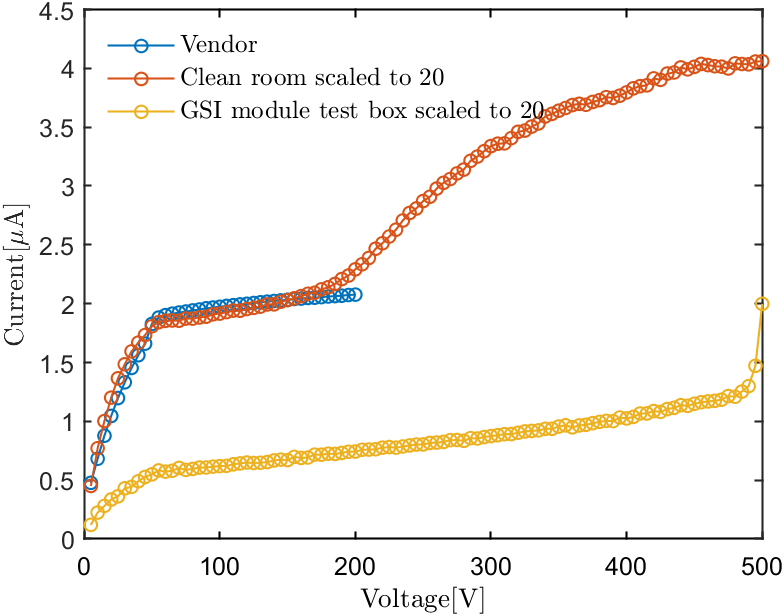
\includegraphics[width=0.5\columnwidth]{Chapter6/DCS/images/IV/30304Whole.png}
\caption{IV curves of a module}
\label{fig_IV_good}
\end{figure}

\newpage
\subsection{Data rates and leakage current}
Data rates from subsystems contain important information about the detector performance. Figure~\ref{fig_data_rates_Ag} shows an example of the \gls{mSTS} operation during data-taking with \footnote{gold beam colliding with gold target}{Au+Au} system ($T= 1~\mathrm{AGeV}$) and later with Ni+Ni system (without the \gls{mSTS}). Data rates are clearly correlated with the beam intensity. Regardless of the beam intensities, the \gls{mSTS} (with the chosen settings) is responsible for more than half of the total data. During the beam intensities of $10^{8}$ ions/s, \gls{mSTS}'s data rate was about 500 MB/s and with the maximum beam intensities it was up to 2000 MB/s, reaching the limits \gls{FEB}s uplink. 
\begin{figure}[H]
\centering
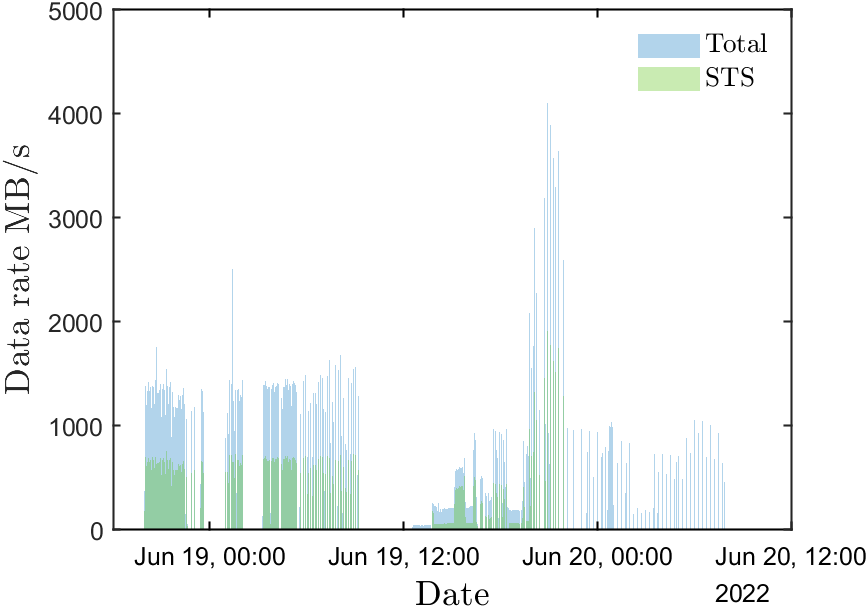
\includegraphics[width=0.55\columnwidth]{Chapter6/DCS/images/rates/Ag_total.png}
\caption{Data rates of all the \gls{mSTS} units in comparison to the overall data rate of all subsystems during data-taking}
\label{fig_data_rates_Ag}
\end{figure}
\newpage
There is a direct correlation of data rates with the leakage current increase, what can be seen in figure~\ref{fig_Data}. This correlation gives more insight into the operation and state of the silicon sensors.
\begin{figure}[!h]
\centering
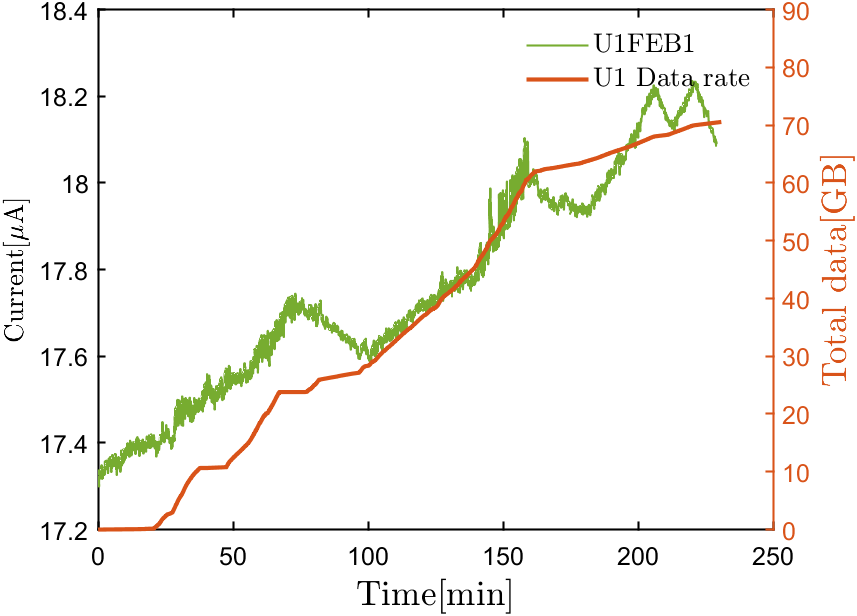
\includegraphics[width=0.45\columnwidth]{Chapter6/DCS/images/U1_data_rate.png}
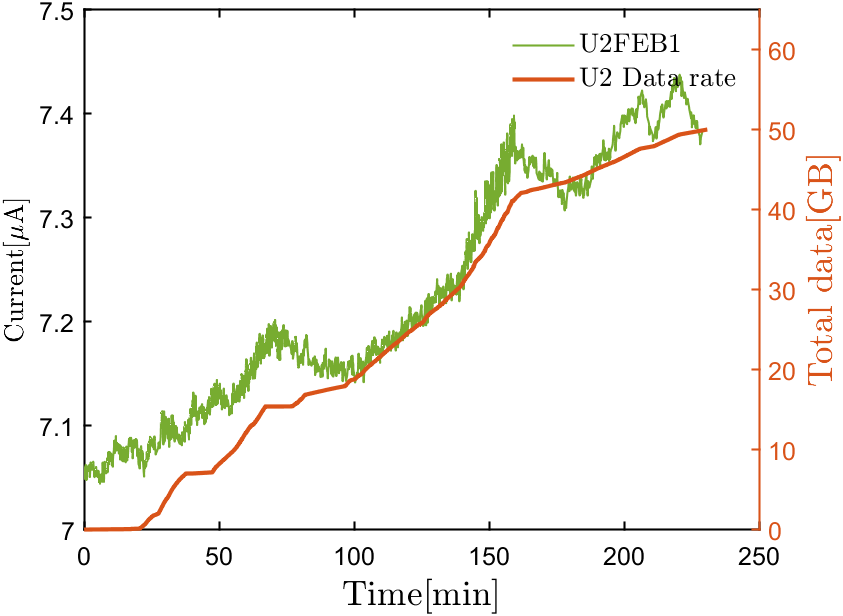
\includegraphics[width=0.45\columnwidth]{Chapter6/DCS/images/U2_data_rate.png}
\caption{Leakage current evolution of the \gls{mSTS} silicon sensors and respective integrated data rate}
\label{fig_Data}
\end{figure}

\section{Conclusions}

The successful operation of the \gls{mSTS}, including the \gls{DCS} and \gls{DAQ} chain set an important milestone toward completion of the \gls{STS} project. The first extensive data-taking activities with two tracking stations proved the general idea behind the assembly of the detector. The prototyping of the supervisory layer of the \gls{mSTS} detector took place and was successfully concluded, proving that the concept was extremely useful, not only for a large detector, accelerator setups but also for smaller experiments. After almost two years of operation of the containers based system proved to be a reliable, easily maintained solution. Nevertheless, for the final system, several additional applications are needed. The \gls{STS} will be much more complex and challenging when it comes to configuration and running. Moreover, it will be extremely important to have both hardware and software interlocking to ensure the machine's safety.

The \gls{mSTS} didn't publish its overall status to any external agent. Due to that reason, some information like \gls{ASIC} internal temperature or $V_{DDM}$ were only accessible via the data acquisition chain (\gls{DCA}-\gls{CRI}). In the future, each subsystem will have an assigned \gls{SCA} to tackle control of the readout chain and the \gls{DCS}. 


Temperature sensors located inside the \gls{mSTS} and information about the current drawn by the sensors indicate the silicon sensors' state. The sensors may degrade over time due to radiation-related bulk damage,  which leads i.a. to leakage current increase, type inversion, etc. Those effects can be partially studied through the \gls{DCS} and the control strategy adopted respectively to the results.

Figure \ref{fig_dcs_results} shows the how the \gls{DCS} performed during about 2 years of operation. Due to the radiation-induced soft errors in the controllers of the cooling units, there were several occasions that the operation of the \gls{STS} needed to be halted. Usually, such an interruption in the operation was automatically triggered by the \gls{FSM}. Nevertheless, listed errors might also include the intervention in the system. In that case the error related to the cooling system was logged, but the FSM might have been off.
\begin{figure}[!h]
\centering
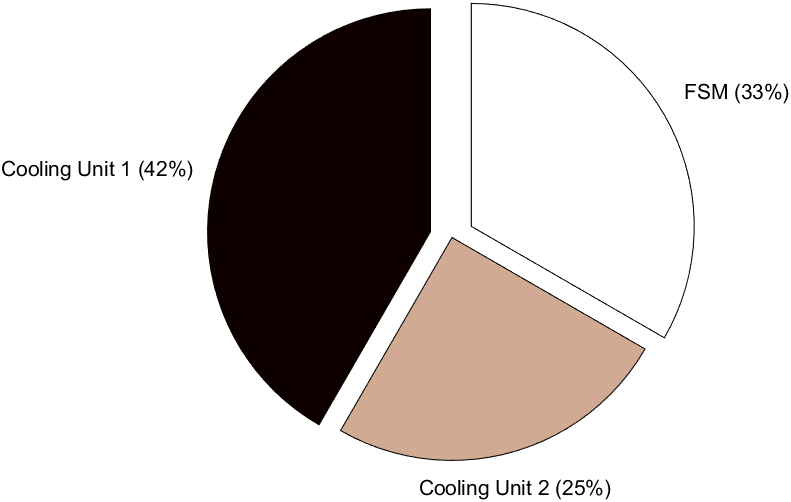
\includegraphics[width=0.55\columnwidth]{Chapter6/DCS/images/DCSpie.png}
\caption{Results from the operation}
\label{fig_dcs_results}
\end{figure}
